\Chapter{A szállítási probléma formalizálása}

\Section{A kiszállítási probléma általános modellje}

Vizsgált esetek:

étterem: egy - több
futár: egy - több
kiszállítás: egy - több

(1, 1, 1)
(1, 1, *)
(*, 1, *)
(1, *, *)
(*, 1, *)
(*, *, *)

\Section{Utazóügynök probléma}

Egy futár, több kiszállítás esete.

Összes lehetséges út:
\[
\dfrac{(n-1)!}{2}
\]
Ezek közül kell választanunk, ez ugyanis a Hamilton-körök száma az n pontú teljes gráfban.

A képlet csak $n > 2$ esetén működik.

Ezen importok szükségesek a szimuláció futtatásához

\begin{python}
from scipy.spatial import distance_matrix
\end{python}

A cél az, hogy listát készítsünk a pontokról, amelyek mindegyike két koordinátát tartalmaz $(x, y)$, amelyek 0 és 100 közötti véletlen egész számokként kerülnek kiválasztásra. Jelen esetben 10 ilyen pont lesz.

\begin{python}
points = [random.sample(range(100), 2) for x in range(10)]
\end{python}

A pontok közötti távolságok kimutatását így oldottam meg.

\begin{python}
data = Points
points = ['1', '2', '3', '4', '5', '6', '7', '8', '9', '10'] \\
df = pd.DataFrame(data, columns=['xcord', 'ycord'], index=points) \\
pd.DataFrame(distance_matrix(df.values, df.values), index=df.index, columns=df.index)}
\end{python}

Ezt a kimenetett adta válaszul.

\begin{figure}[h!]
\centering
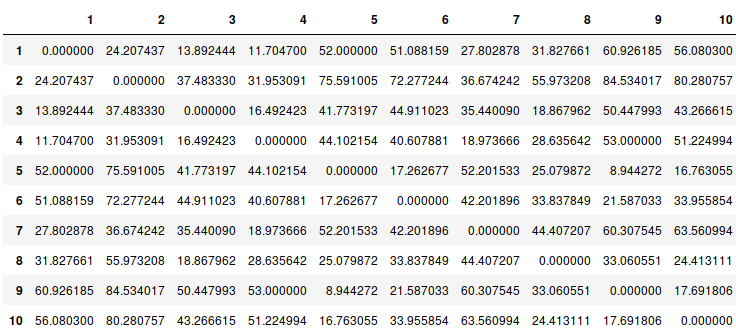
\includegraphics[width=\textwidth]{images/table.png}
\caption{Kimenet}
\label{fig:kimenet}
\end{figure}

A travel egy 10 számból álló lista, amely a pontok meglátogatására utal. Feltételezzük, hogy zárt hurokra van szükség, így az utolsó pont autómatikusan csatlakozik az elsőhöz.


\begin{python}
travel = random.sample(range(10), 10);}
\end{python}

Elindítunk egy ciklust az adott értékekkel


\begin{python}
for tlp in numpy.logspace(0, 5, num = 100000)[::-1]:
\end{python}


Két pont véletlenszerű cseréjével új új utat képzünk. Úgy valósítom meg, hogy választok két számot az i-t és a j-t. Összeállítom a newTravel-t a régi travel másolásával az i indexig, majd összefűzöm a j-edik travelel-t és egészen folytatom addig, amíg a j nem éri el az i-edik pontot, majd befejezem a travel többi részét.


\begin{python}
[i, j] = sorted(random.sample(range(10), 2)); \\
newTravel = travel[:i] + travel[j:j + 1] + travel[i + 1:j] + travel[i:i + 1] + travel[j + 1:]
\end{python}


Ha az if értéke igaz akkor a travel megkapja a newTravel értékét, az előzöekben említett csere miatt ez már változott. Az elképzelés az, hogy minimalizálni szeretnénk a pontok közti távolságok költségének összegét. Ehhez a Gibb-s faktor-t használtam fel, aminek lényege, az új állapotba való átmenet valószínűsége. Csak az i-edik és j-edik pontok közötti távolságokat szükséges összegezni, mivel a többi távolság ugyanaz mint a travel-ben mint a newTravel-ben egyaránt. Ha a faktor > 1 akkor az új költség alacsonyabb, travel megkapja a newTravel értékét.


\begin{python}
traveld = sum([math.sqrt(sum( [(points[travel[(k + 1) % 10]][d] - points[travel[k \% 10]][d]) **  2 for d in [0, 1]])) for k in [j, j - 1, i, i - 1]])
    newTraveld = sum([math.sqrt(sum([(points[newTravel[(k + 1) % 10]][d] - points[newTravel[k \% 10]][d]) ** 2 for d in [0, 1]])) for k in [j, j - 1, i, i - 1]])
    if math.exp((traveld - newTraveld) / tlp) > random.random():
        travel = copy.copy(newTravel);
\end{python}        


Az algoritmus végeztével már csak meg kell jeleníteni a kívánt pontokat, ez kirajzol egy gráfot, amely optimális utat ad. Ehhez a pyplot libary-t használtam


\begin{python}
plt.plot([points[travel[i % 10]][0] for i in range(11)], [points[travel[i \% 10]][1] for i in range(11)], 'xb-')
plt.show()
\end{python}

A következő gráfok megmutatják a kívánt utat vároksok száma szerint. Mivel véletlenszerű számok összehasonlításán alapszik az algoritmus ezáltal az összehasonlítások száma igen magas, viszont stagnál bizonyos értékek között.

% TODO: A képeket egy oldalra, táblázatos formába összerakni!

5 város esetén
Összehasonlítások száma: 74 434
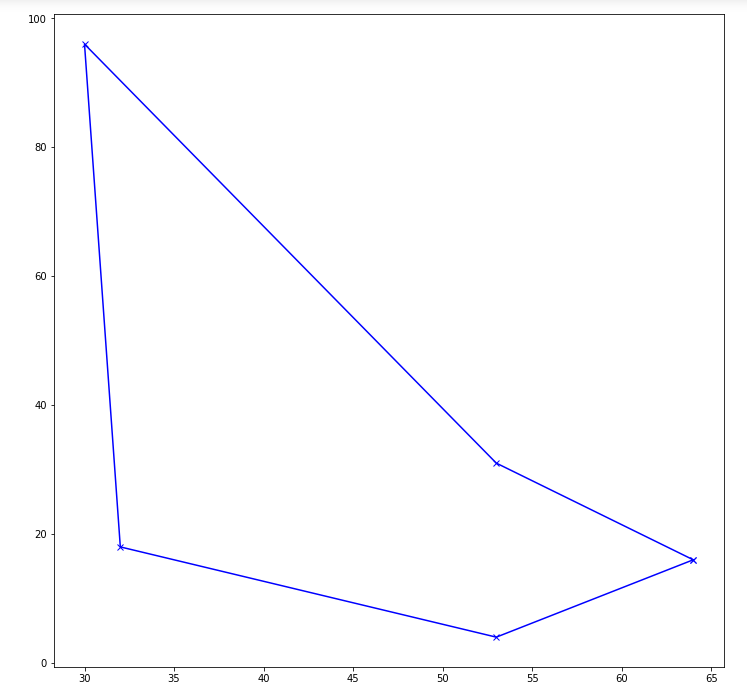
\includegraphics[scale=0.4]{images/5.png}

10 város esetén
Összehasonlítások száma: 68 594
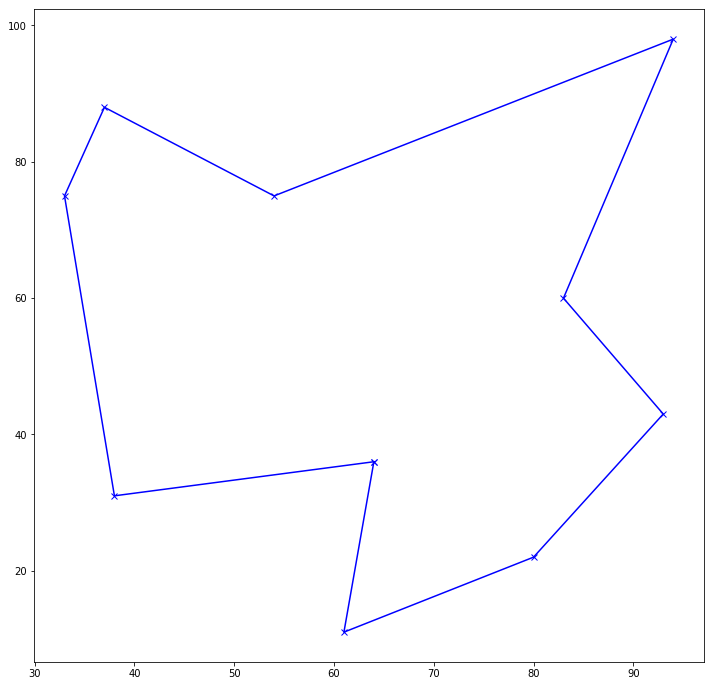
\includegraphics[scale=0.4]{images/10.png}

15 város esetén
Összehasonlítások száma: 66 672
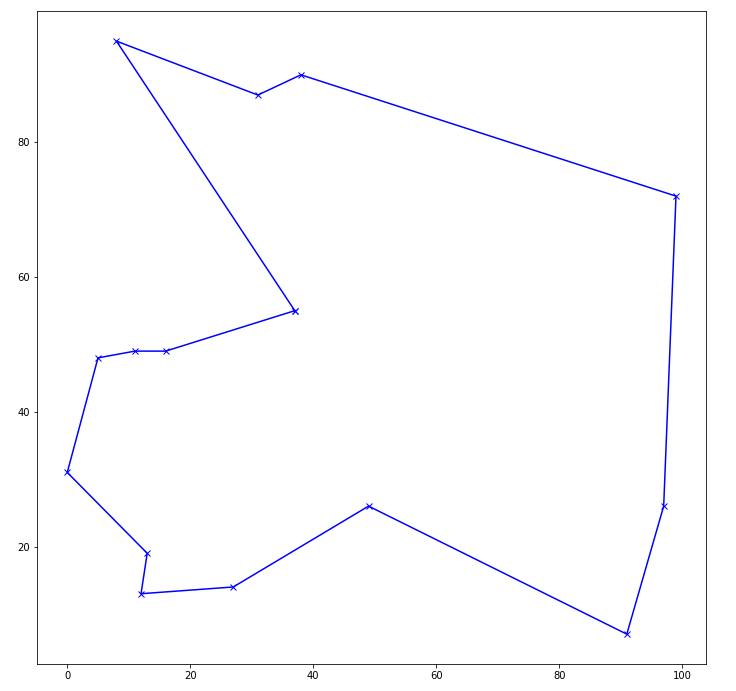
\includegraphics[scale=0.4]{images/15.png}

20 város esetén
Összehasonlítások száma: 65 265
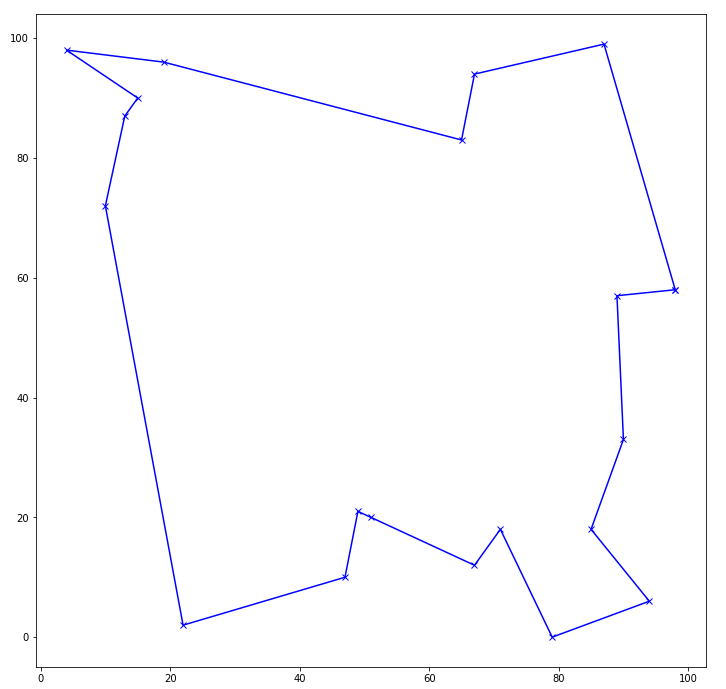
\includegraphics[scale=0.4]{images/20.png}

25 város esetén
Összehasonlítások száma: 67 865
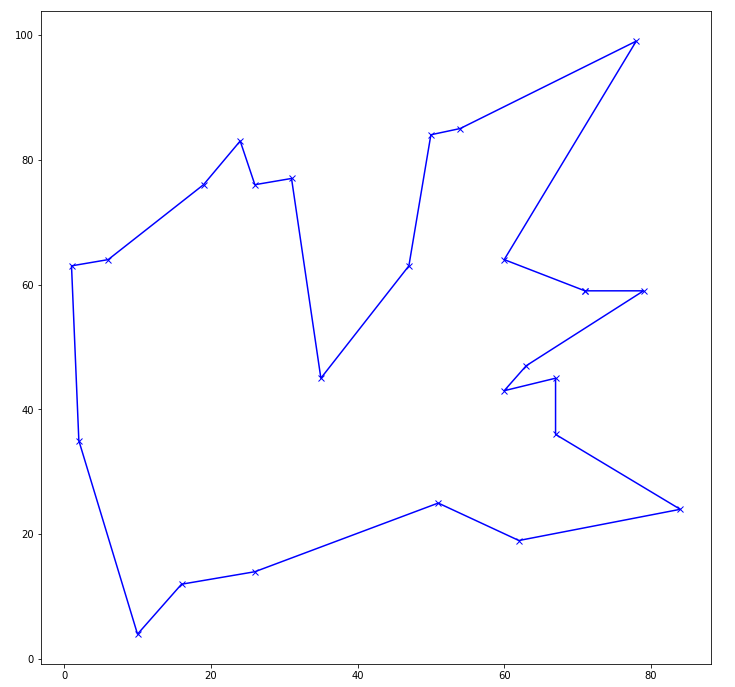
\includegraphics[scale=0.4]{images/25.png}

30 város esetén
Összehasonlítások száma: 65 324
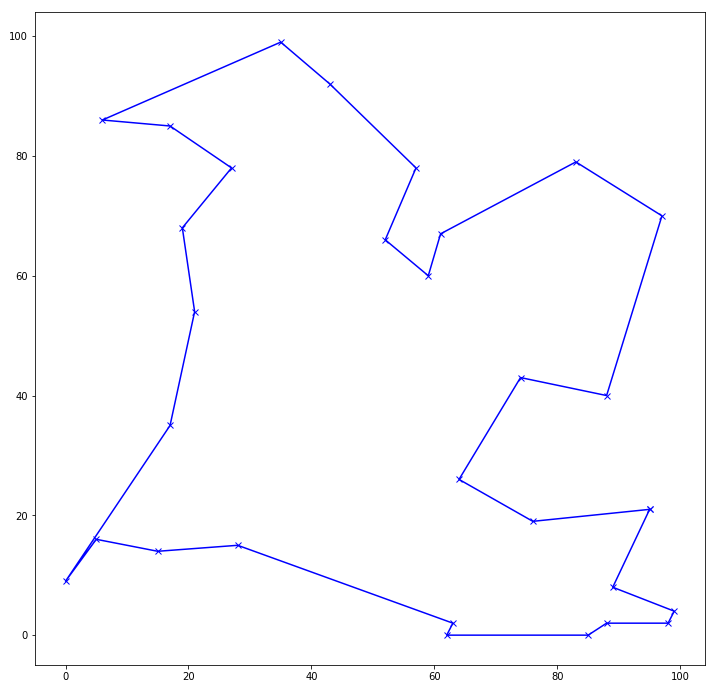
\includegraphics[scale=0.4]{images/30.png}

35 város esetén
Összehasonlítások száma: 67 230
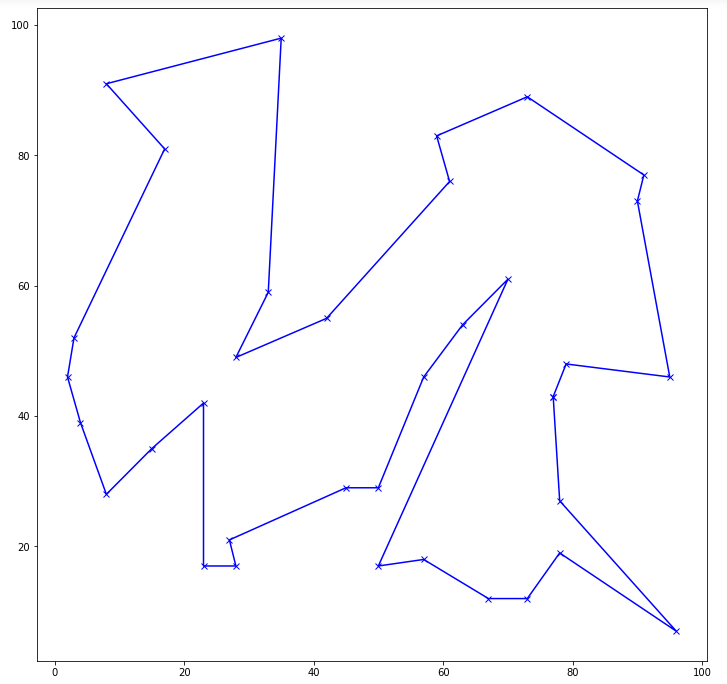
\includegraphics[scale=0.4]{images/35.png}

40 város esetén
Összehasonlítások száma: 66 008
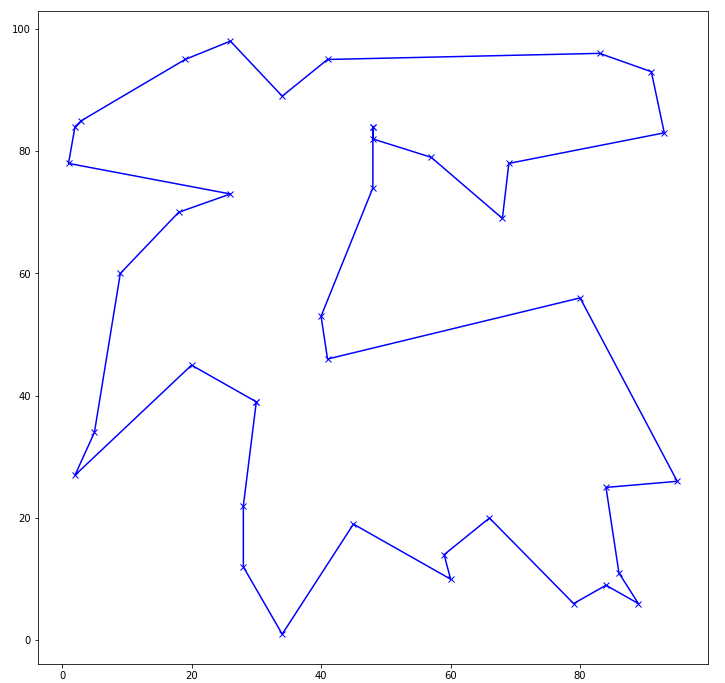
\includegraphics[scale=0.4]{images/40.png}

Több lefuttatott teszt után is megfgyelhető, hogy az összehasonlítások száma 65 ezer és 75 ezer között mozog. Egytől egyig az optimális utat adták.
